\chapter{Deployment and Operations}

\section{Execution Models}
The repository supports two practical execution models:
\begin{enumerate}[leftmargin=2em]
\item \textbf{Dual-namespace model}: both server and client run in separate namespaces.
\item \textbf{Host-server model}: server runs on host, client runs in namespace (for easier internet NAT).
\end{enumerate}

Scripts suggest both models are used for different troubleshooting and internet-access scenarios.

\section{Baseline Setup Procedure}
A canonical setup path from repository assets:
\begin{enumerate}[leftmargin=2em]
\item Install Python dependencies via \texttt{pip install -r requirements.txt}.
\item Generate synchronized client/server configs via \texttt{generate\_config.py}.
\item Initialize namespaces via \texttt{scripts/netns\_setup.sh}.
\item Start server then client in target execution contexts.
\item Validate tunnel reachability with ping to \texttt{10.8.0.1}.
\end{enumerate}

\section{Operational Runbook Table}
\begin{table}[H]
\centering
\caption{Operational Commands and Purpose}
\begin{tabular}{p{0.42\textwidth}p{0.44\textwidth}}
\toprule
\textbf{Command Pattern} & \textbf{Purpose} \\
\midrule
\texttt{python3 generate\_config.py} & Create fresh synchronized configs \\
\texttt{sudo bash scripts/netns\_setup.sh} & Build client/server namespace topology \\
\texttt{sudo ip netns exec vpn-server ...server.py} & Start server in namespace \\
\texttt{sudo ip netns exec vpn-client ...client.py} & Start client in namespace \\
\texttt{sudo bash scripts/server\_nat.sh} & Configure NAT and forwarding \\
\texttt{sudo bash scripts/diagnose.sh} & Automated diagnostics for connectivity \\
\bottomrule
\end{tabular}
\end{table}

\section{NAT and Internet Access Path}
Internet access from the VPN client is achieved through host NAT rules. The script configures:
\begin{itemize}[leftmargin=2em]
\item \texttt{net.ipv4.ip\_forward=1}
\item \texttt{iptables -t nat POSTROUTING MASQUERADE}
\item FORWARD rules between tunnel and host egress interface
\item Namespace DNS configuration under \texttt{/etc/netns/vpn-client/resolv.conf}
\end{itemize}

\begin{figure}[H]
\centering
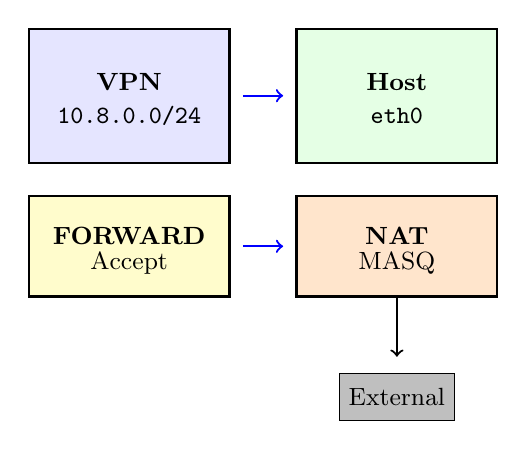
\begin{tikzpicture}[scale=0.85, every node/.style={font=\small}]
  % VPN Subnet
  \draw[thick, fill=blue!10] (0.5,5) rectangle (3.5,7);
  \node at (2,6.2) {\textbf{VPN}};
  \node at (2,5.7) {\texttt{10.8.0.0/24}};
  
  % Iptables FORWARD
  \draw[thick, fill=yellow!20] (0.5,3) rectangle (3.5,4.5);
  \node at (2,3.9) {\textbf{FORWARD}};
  \node at (2,3.5) {\small Accept};
  
  % NAT POSTROUTING
  \draw[thick, fill=orange!20] (4.5,3) rectangle (7.5,4.5);
  \node at (6,3.9) {\textbf{NAT}};
  \node at (6,3.5) {\small MASQ};
  
  % Host Interface
  \draw[thick, fill=green!10] (4.5,5) rectangle (7.5,7);
  \node at (6,6.2) {\textbf{Host}};
  \node at (6,5.7) {\texttt{eth0}};
  
  % Flow arrows
  \draw[->, thick, blue] (3.7,6) -- (4.3,6);
  \draw[->, thick, blue] (3.7,3.75) -- (4.3,3.75);
  
  % Destination
  \node[draw, fill=lightgray, minimum height=0.6cm] at (6,1.5) {External};
  \draw[->, thick] (6,3) -- (6,2.1);
\end{tikzpicture}
\caption{NAT and Forwarding Configuration}
\end{figure}

\section{Diagnostics Workflow}
\texttt{scripts/diagnose.sh} provides a useful fault-isolation checklist:
\begin{enumerate}[leftmargin=2em]
\item Verify namespaces exist.
\item Verify \texttt{tun0} presence and address.
\item Test tunnel ping.
\item Inspect routes and DNS configuration.
\item Check forwarding and NAT rules.
\item Test external reachability and optional HTTP response.
\end{enumerate}

This script-driven checklist lowers debugging time and creates a reproducible support process.

\section{Operational Risks Observed in Scripts}
From static review, operations scripts include a few consistency risks:
\begin{itemize}[leftmargin=2em]
\item Variable scope assumptions in NAT script (client namespace variable reference).
\item Cleanup argument handling appears near script tail in some files.
\item Mixed assumptions about server location (host vs namespace) across helper scripts.
\end{itemize}

These are manageable but should be normalized to avoid user confusion.

\section{Hardening the Operational Surface}
Recommended improvements:
\begin{enumerate}[leftmargin=2em]
\item Add strict mode in shell scripts: \texttt{set -euo pipefail}.
\item Centralize shared script variables in one sourced file.
\item Make cleanup handlers early and idempotent.
\item Emit explicit mode banner: \texttt{host-server} vs \texttt{dual-namespace}.
\item Add script tests in CI using containerized Linux testbeds.
\end{enumerate}

\section{Observability}
Current observability is log-centric with periodic stats from Python processes. Operational maturity can be improved with:
\begin{itemize}[leftmargin=2em]
\item Structured logging fields (namespace, endpoint role, flow direction).
\item Exportable counters (Prometheus textfile, JSON snapshots).
\item Optional packet trace mode for controlled debugging.
\end{itemize}

\section{Deployment Profiles}
\begin{table}[H]
\centering
\caption{Suggested Deployment Profiles}
\begin{tabular}{p{0.27\textwidth}p{0.24\textwidth}p{0.35\textwidth}}
\toprule
\textbf{Profile} & \textbf{Primary Goal} & \textbf{Recommended Settings} \\
\midrule
Learning lab & Concept demonstration & Dual namespace, verbose logs, debug scripts \\
Classroom demo & Reliable reproducibility & Host-server mode, prebuilt configs, scripted launch \\
Research prototype & Extend architecture & Add packet IDs, benchmark hooks, profile tooling \\
\bottomrule
\end{tabular}
\end{table}

\section{Takeaway}
WhisperTunnel's operational tooling is unusually rich for an educational repository. It already enables realistic demonstrations and debugging workflows, and with script normalization it can provide near turnkey lab reproducibility.
